برای راه‌اندازی pgp 
مراحل زیر را دنبال می‌کنیم. قابل ذکر است که سیستم‌عامل ما 
\lr{Ubuntu 22.04}
می‌باشد. ابتدا برای نصب از دستور زیر استفاده می‌کنیم :
\begin{latin}
    \begin{lstlisting}
apt install gap gnupg2
    \end{lstlisting}
\end{latin}
سپس باید جفت کلید خود را جنریت کنیم.
\begin{center}
    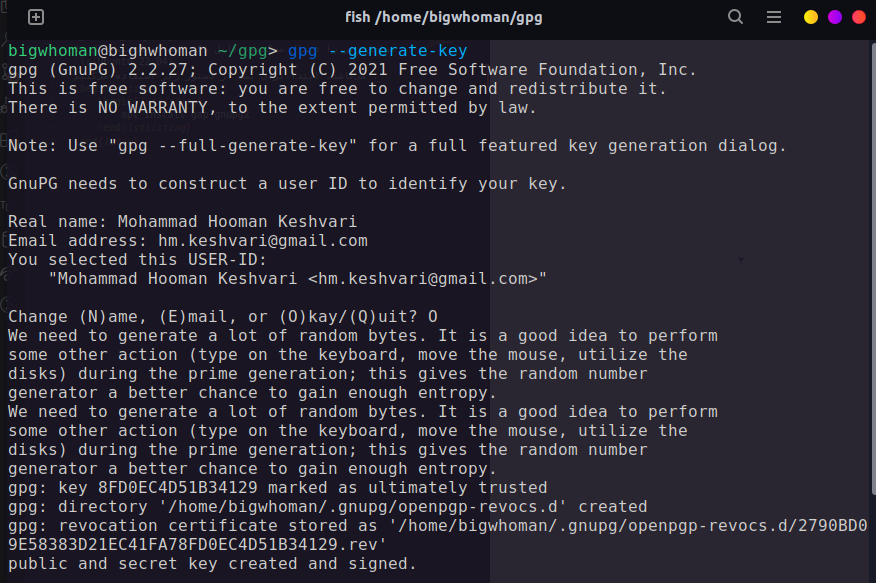
\includegraphics[scale=0.5]{pics/pgp1.png}
\end{center}

بعد از جنریت کردن جفت‌ کلیدهای خود، باید کلید عمومی را با زدن دستور زیر import کنیم.
\begin{latin}
    \begin{lstlisting}
gpg --import Reza_0xCFBEEE88_public.asc
\end{lstlisting}
\end{latin}

سپس با زدن دستورات زیر ابتدا 
\lr{plain text}
را امضا کرده و سپس آنرا encrypt 
می‌کنیم.


\begin{center}
    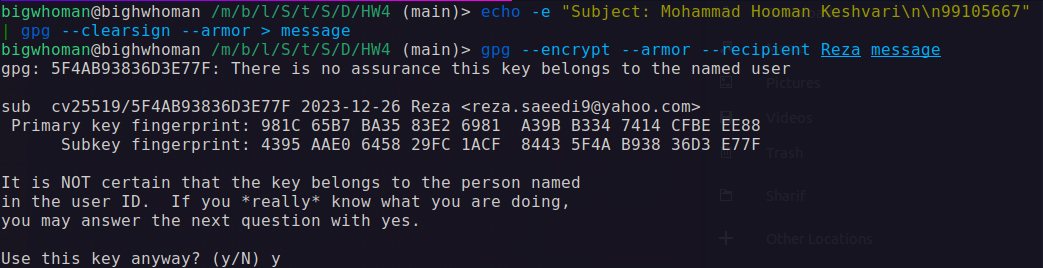
\includegraphics[scale=0.47]{pics/pgp_encrypt.png}
\end{center}
با دستورات بالا یک فایل message.asc 
ساخته می‌شود که حاوی پیام و امضا شده آن است که در سمت گیرنده با دستور زیر می‌توان به خود پیام رسید.
\begin{latin}
    \begin{lstlisting}
gpg --decrypt --output message.txt message.asc
\end{lstlisting}
\end{latin}

در صورتی که امضا درست باشد باید با زدن دستور زیر خروجی مانند خروجی زیر را مشاهده کنید.

ساخته می‌شود که ابتدا باید مطمئن شویم درست امضا شده :
\begin{center}
    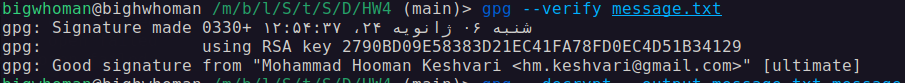
\includegraphics[scale=0.5]{pics/pgp3.png}
\end{center}

با زدن دستور زیر نیز کلید عمومی خود را در فایل 
\lr{keshvari.asc}
قرار می‌دهیم و آنرا به ایمیل ضمیمه می‌کنیم.


\begin{latin}
    \begin{lstlisting}
gpg --armor --output keshvari.asc --export "Mohammad Hooman Keshvari"
\end{lstlisting}
\end{latin}